\documentclass{sig-alternate}

%------------------------------------------------------------------------------- 
% Math packages
%------------------------------------------------------------------------------- 

% The "amsmath" package provides advanced math extensions.
\usepackage{amsmath}

% The "amssymb" package adds new symbols to be used in math mode.
\usepackage{amssymb}

% The "amsthm" package adds the "proof" environment and "theoremstyle" command.
% \usepackage{amsthm}

% The "faktor" package adds the "faktor" macro for variable substitution (i.e. vulgar fractions). This depends on the "amssymb" package.
% \usepackage{faktor}

% The "semantic" package adds new macros for (PL-style) inference rules.
% \usepackage[inference]{semantic}

%------------------------------------------------------------------------------- 
% Figure packages
%------------------------------------------------------------------------------- 

% The "fancyvrb" package provides advanced customization of verbatim environments, such as font families, numbering lines, box borders etc.
% \usepackage{fancyvrb}

% The "graphicx" package allows including external graphic files.
\usepackage{graphicx}

% The "subfig" package allows multiple sub-figures within a single figure, where sub-figures can be separately captioned and labeled, e.g. Figure % 1.2(a). This is a replacement for the older "subfigure" package.
%\usepackage{subfig}

% Replaced the "subfig" package with the "subcaption" package
\usepackage{subcaption}

% HACK: The caption package (included by the subfig package) requires a counter for ACM's copyright box.
\newcounter{copyrightbox}

% The "float" package allows the "H" option for figures, which places a float % at a precise location.
\usepackage{float}

% The "caption" package allows captions for figures that are not actually in a floating environment (e.g. framed environment).
\usepackage{caption}

% The "mdframed" package creates framed regions that can break across pages.
\usepackage{mdframed}


% The "algorithm2e" package provides keywords for typesetting algorithms. The "noend" option disables the printing of the "end" keywords. Use "algomargin" to decrease the margins for all algorithms.

% Kevin: To resolve conflict of algorithm2e with other packages, a common problem with ACM template.
% See http://ergodicthoughts.blogspot.com/2009/06/latex-too-many-s-algorithm2e.html
% \makeatletter
% \newif\if@restonecol
% \makeatother
% \let\algorithm\relax
% \let\endalgorithm\relax
% \usepackage[noend,boxed]{algorithm2e}
% \setlength{\algomargin}{0.5em}

%------------------------------------------------------------------------------- 
% Layout packages
%------------------------------------------------------------------------------- 

% The "multirow" package allows table cells to span more than one row.
\usepackage{multirow}

% The "balance" package allows columns of the last page to be of equal height.
\usepackage{balance}

% The "fixltx2e" package prevents two-column figures from being placed out-of-order wrt regular (one-column) figures. 
% \usepackage{fixltx2e} 

% The "dblfloatfix" package allows two-column figures to be placed at the page's bottom. 
% \usepackage{dblfloatfix}

%------------------------------------------------------------------------------- 
% Whitespace packages
%------------------------------------------------------------------------------- 

% The "savetrees" package saves space on a page.
% \usepackage[all=normal,paragraphs=tight,floats=tight,bibnotes=tight]{savetrees}
% \usepackage[all=normal,paragraphs=tight,floats=tight,bibnotes=tight,bibliography=tight]{savetrees}

% The "setspace" package allows changing the inter-line spacing to be a multiple of the default line spacing.
% \usepackage{setspace}
% \setstretch{0.98}

% The "titlesec" package allows changing the whitespace around section headings.
% \usepackage[compact]{titlesec}

%------------------------------------------------------------------------------- 
% Font packages
%------------------------------------------------------------------------------- 

% The "beramono" package provides Bitstream Vera Mono, which has a bold typewritter fontface.
\usepackage[scaled]{beramono}
\usepackage[T1]{fontenc}

% The "courier" package provides Courier, which has a bold typewritter fontface.
%\usepackage{courier}

% The "upquote" package fixes tilde and quote in verbatim environments.
\usepackage{upquote}

%------------------------------------------------------------------------------- 
% Misc packages
%------------------------------------------------------------------------------- 

% The "optional" package allows multiple versions of the document via optional text.
\usepackage{optional}

% The "xstring" package allows switch/case conditionals.
\usepackage{xstring}

% The "xcolor" package allows colored text and backgrounds.
\usepackage[table]{xcolor}

% The "soul" package allows highlighting.
\usepackage{soul}

% The "ulem" package allows highlighting.
\usepackage[normalem]{ulem}

% The "tocloft" packages allows generating custom lists that are similar to table of contents, list of figures etc.
% \usepackage[subfigure]{tocloft}

% The "hyperref" package allows creating hyperlinks. Note that it must be the last package loaded, and will automatically includes the "url" package.
\usepackage{hyperref}

% The "hypcap" package fixes "hyperref" so that hyperlinks go to the top of a float (as opposed to its caption).
\usepackage[all]{hypcap}

%------------------------------------------------------------------------------- 
% Whitespace
%------------------------------------------------------------------------------- 

% Adjust whitespace above and below captions
% \addtolength{\abovecaptionskip}{-5pt}
% \addtolength{\belowcaptionskip}{-9pt}

% Adjust whitespace before/after floats
% \setlength{\textfloatsep}{10pt plus 1.0pt minus 2.0pt}
% \setlength{\floatsep}{6pt plus 1.0pt minus 1.0pt}

%------------------------------------------------------------------------------- 
% Macros
%------------------------------------------------------------------------------- 

% Define our own compact enumerate
\newenvironment{compact_enum}
{\setlength{\leftmargini}{1em}
\begin{enumerate}
  \setlength{\labelsep}{.3em} 
  \setlength{\itemsep}{.4em}
  \setlength{\parskip}{0pt}
  \setlength{\parsep}{0pt}}
{\end{enumerate}}

% Define our own compact itemize
\newenvironment{compact_item}
{\setlength{\leftmargini}{1em}
\begin{itemize}
  \setlength{\labelsep}{.3em} 
  \setlength{\itemsep}{.4em}
  \setlength{\parskip}{0pt}
  \setlength{\parsep}{0pt}}
{\end{itemize}}

% \newtheorem{theorem}{Theorem}[section]
% \newtheorem{lemma}[theorem]{Lemma}
% \newtheorem{proposition}[theorem]{Proposition}
% \newtheorem{corollary}[theorem]{Corollary}

% \newenvironment{proof}[1][Proof]{\begin{trivlist}
% \item[\hskip \labelsep {\bfseries #1}]}{\end{trivlist}}
% \newenvironment{definition}[1][Definition]{\begin{trivlist}
% \item[\hskip \labelsep {\bfseries #1}]}{\end{trivlist}}
% \newenvironment{example}[1][Example]{\begin{trivlist}
% \item[\hskip \labelsep {\bfseries #1}]}{\end{trivlist}}
% \newenvironment{remark}[1][Remark]{\begin{trivlist}
% \item[\hskip \labelsep {\bfseries #1}]}{\end{trivlist}}

% \newcommand{\qed}{\nobreak \ifvmode \relax \else
%       \ifdim\lastskip<1.5em \hskip-\lastskip
%       \hskip1.5em plus0em minus0.5em \fi \nobreak
%       \vrule height0.75em width0.5em depth0.25em\fi}


%------------------------------------------------------------------------------- 
% Database symbols
%------------------------------------------------------------------------------- 

\def\join{$\bowtie$}
\def\ojoin{\setbox0=\hbox{$\bowtie$}%
  \rule[-.02ex]{.25em}{.4pt}\llap{\rule[\ht0]{.25em}{.4pt}}}
\def\leftouterjoin{\mathbin{\ojoin\mkern-5.8mu\bowtie}}
\def\rightouterjoin{\mathbin{\bowtie\mkern-5.8mu\ojoin}}
\def\fullouterjoin{\mathbin{\ojoin\mkern-5.8mu\bowtie\mkern-5.8mu\ojoin}}
\def\semijoin{\mbox{$\mathrel{\raise1pt\hbox{\vrule height5pt depth0pt\hskip-1.5pt$>$\hskip -2.5pt$<$}}$}}
\def\antisemijoin{\overline{\semijoin}}

%------------------------------------------------------------------------------- 
% Grammar symbols (BNFs and Tree Grammars) 
%------------------------------------------------------------------------------- 

% Formatting commands for tree grammars
\newcommand{\gn}[1]  {\textit{#1}}              % (N)on-terminal
\newcommand{\gt}[1]  {\textbf{#1}}              % (T)erminal
\newcommand{\gl}[1]  {\texttt{\textbf{#1}}}     % (L)iteral
\newcommand{\gs}[1]  {\textit{#1}}              % (S)pecial construct
\newcommand{\gp}[0]  {$\rightarrow$}            % (P)roduction rule
\newcommand{\gd}[0]  { $|$ }                    % (D)isjunction


% Use either package to make commentary public or private. If commentary is
% private, they will also be stripped by arxiv-sanitize.sh.
\usepackage{commentary-public}
%\usepackage{commentary-arxiv-private}
\usepackage{tabularx}
\usepackage{caption,subcaption}																																		
% Prodromou: Use for comments during collaboration. Turn off by uncommenting "remarkfalse"
\newif\ifremark
\long\def\remark#1{
\ifremark%
        \begingroup%
        \dimen0=\columnwidth
        \advance\dimen0 by -1in%
        \setbox0=\hbox{\parbox[b]{\dimen0}{\protect\em #1}}
        \dimen1=\ht0\advance\dimen1 by 2pt%
        \dimen2=\dp0\advance\dimen2 by 2pt%
        \vskip 0.25pt%
        \hbox to \columnwidth{%
                \vrule height\dimen1 width 3pt depth\dimen2%
                \hss\copy0\hss%
                \vrule height\dimen1 width 3pt depth\dimen2%
        }%
        \endgroup%
\fi}

\remarktrue
%\remarkfalse																																														
\usepackage{hhline}
%\usepackage{amsmath}
% \usepackage{commentary-arxiv-private}https://preview.overleaf.com/public/zckgmbcqqxpd/images/f848aee704bdc6b4fb1a2d1d3c4a093089841ee3.jpeg

% ACM: Package to generate and customize Algorithm as per ACM style
% The "noend" option disables the printing of the "end" keywords. Use "algomargin" to decrease the margins for all algorithms.
\usepackage[ruled, linesnumbered]{algorithm2e}
\renewcommand{\algorithmcfname}{ALGORITHM}
\SetAlFnt{\small}
\SetAlCapFnt{\small}
\SetAlCapNameFnt{\small}
\SetAlCapHSkip{0pt}
\usepackage{paralist}
\usepackage{fancyvrb}
\usepackage{listings, multicol}

% Use one of the packages below to produce a document version. If a version
% ends with "-private", all other unnecessary text will be stripped by
% arxiv-sanitize.sh.
%\usepackage{version-conference}                % Conference version
\usepackage{version-extended-arxiv-private}    % Extended version (with all other text stripped, so that the source can be uploaded to arXiv)
%\usepackage{version-extended-draft}            % Extended + Draft version
%\usepackage{version-all}                       % All text side-by-side with color highlighting

%------------------------------------------------------------------------------- 
% Macros
%------------------------------------------------------------------------------- 

\IncMargin{-\parindent}

% Toggle between two versions: Basic vs Extended
\def\UseOption{basic}
% \def\UseOption{extended}
\newcommand{\toggle}[2]{\opt{basic}{#1}\opt{extended}{#2}}

% Column types
\newcolumntype{B}{|@{~}r@{~}|l@{~}c@{~~~}l@{~}|}    % (B)NF

% Code examples
\DefineVerbatimEnvironment{code}{Verbatim}{commandchars=\\\{\},frame=single,numbers=left,fontsize=\scriptsize}

% Template directives 
\newcommand{\directive}[2]{%
\ifx&#2&%
\textbf{<\% #1 \%>}%
\else%
\textbf{<\% #1}{ #2 }\textbf{\%>}%
\fi%
}

% Paths
\newcommand{\pp}[1]{\ensuremath{\hat{#1}}}
\newcommand{\contains}{\ensuremath{\supseteq}}

% Diffs
\newcommand{\diff}[3]{\ensuremath{\Delta^{#1}_{#2}(#3)}}
\newcommand{\insertarray}[1]{\diff{\operatorname{insert}}{\operatorname{array}}{#1}}
\newcommand{\insertbag}[1]{\diff{\operatorname{insert}}{\operatorname{bag}}{#1}}
\newcommand{\inserttuple}[1]{\diff{\operatorname{insert}}{\operatorname{tuple}}{#1}}
\newcommand{\append}[1]{\diff{\operatorname{append}}{\operatorname{array}}{#1}}
\newcommand{\update}[1]{\diff{\operatorname{update}}{}{#1}}
\newcommand{\delete}[1]{\diff{\operatorname{delete}}{}{#1}}
%\newcommand{\construct}[1]{\diff{\operatorname{construct}}{}{#1}}
%\newcommand{\destruct}[1]{\diff{\operatorname{destruct}}{}{#1}}
\newcommand{\construct}[1]{\diff{\operatorname{construct}}{\operatorname{unit}}{#1}}
\newcommand{\constructattach}[1]{\diff{\operatorname{construct\&attach}}{\operatorname{unit}}{#1}}
\newcommand{\destruct}[1]{\diff{\operatorname{destruct}}{\operatorname{unit}}{#1}}
\newcommand{\attach}[1]{\diff{\operatorname{attach}}{\operatorname{unit}}{#1}}
\newcommand{\detach}[1]{\diff{\operatorname{detach}}{\operatorname{unit}}{#1}}
\newcommand{\hpath}[1]{\ensuremath{\vec{#1}}}
\newcommand{\inserthtml}[1]{\diff{\operatorname{insert}}{\operatorname{html}}{#1}}
\newcommand{\appendhtml}[1]{\diff{\operatorname{append}}{\operatorname{html}}{#1}}
\newcommand{\updatehtml}[1]{\diff{\operatorname{update}}{\operatorname{html}}{#1}}
\newcommand{\deletehtml}[1]{\diff{\operatorname{delete}}{\operatorname{html}}{#1}}

\newcommand{\id}[1]{\hat{#1}}
\newcommand{\inst}[1]{I(#1)}
\newcommand{\diffz}[2]{\triangle^{\operatorname{#1}}(#2)}
\newcommand{\insertdiff}[1]{\diffz{insert}{#1}}
\newcommand{\inserttuplediff}[1]{\diffz{insert\_tuple}{#1}}
\newcommand{\insertarraydiff}[1]{\diffz{insert\_array}{#1}}
\newcommand{\appenddiff}[1]{\diffz{append}{#1}}
\newcommand{\attributediff}[1]{\diffz{attribute}{#1}}
\newcommand{\updatediff}[1]{\diffz{update}{#1}}
\newcommand{\deletediff}[1]{\diffz{delete}{#1}}

\newcommand{\highlight}[1]{\noindent\textbf{#1:}}

\def\env{\mathrm{\Gamma}}
\def\ground{\operatorname{Ground}}
\def\nav{\operatorname{Nav}}
\def\iterate{\operatorname{Iter}}
\def\outputarray{\operatorname{Out}^A}
\def\outputvalue{\operatorname{Out}^V}
\def\function{\operatorname{Func}}
\def\applyplan{\operatorname{Plan}}

% Definition environment
\newtheorem{base}{Base}[section]
\newtheorem{definition}[base]{Definition}
\newtheorem{example}[base]{Example}

% Tabular
\definecolor{lightgrey}{RGB}{235,235,235}
\definecolor{cream}{RGB}{255,255,204}
\newcommand\Tstrut{\rule{0pt}{2.6ex}}       % "top" strut
\newcommand\Bstrut{\rule[-0.9ex]{0pt}{0pt}} % "bottom" strut

% ACM: Metadata Information
% \acmVolume{9}
% \acmNumber{4}
% \acmArticle{39}
% \acmYear{2010}
% \acmMonth{3}

% ACM: Copyright
%\setcopyright{acmcopyright}
%\setcopyright{acmlicensed}
%\setcopyright{rightsretained}
%\setcopyright{usgov}
%\setcopyright{usgovmixed}
%\setcopyright{cagov}
%\setcopyright{cagovmixed}

% ACM: DOI
% \doi{0000001.0000001}

% ACM: ISSN
% \issn{1234-56789}


\begin{document}

\newcommand{\projname}[0]{ViDeTTe}
\newcommand{\angular}[0]{AngularJS}
\newcommand{\react}[0]{React}

\title{Jupyter on Steroids}

\maketitle

% \yannis{Test reminder}
 
% \ifconference{CONF}
% \ifextended{EXT}
% \ifdraft{DRAFT}

% Be less strict about word spacing to avoid various \texttt words overflowing the margins
\begin{sloppypar}


\begin{abstract}

Despite the plethora of recently proposed tools and frameworks, common data analysis tasks such as data retrieval, curation and visualization remain laborious and non-trivial. The limited flexibility of existing frameworks, pushes code-literate data analysts to interactive notebooks such as Jupyter. 

In this work, we argue that interactive notebooks are suboptimal for commonly performed tasks, with regards to their ease of use and interactivity. We propose \projname , a framework designed to facilitate data analysis through the utilization of a template language. We implement a sample data analysis work flow and present the benefits of using {\projname} instead of commonly used imperative language in iPython and Jupyter notebooks.

\end{abstract}




\begin{abstract}




\remark{This abstract is way too long. Most of it should be in the introduction. We should try to keep it under half column with a flow like: issue -> "This paper proposes..." -> Results if any.}
A plethora of tools and frameworks has been proposed, by the database and systems community, for streamlining the admittedly arduous tasks of data retrieval, data curation and data visualization. Since these tasks, typically, have to be carried out in most data science projects, a significant portion of the afore-mentioned tools, focuses on providing a user-friendly way for performing them. Despite the very promising results, however, these tools often seem to limit flexibility as they only focus either on a predetermined set of use/analysis-cases or on only a small fraction of tasks of a typically much bigger pipeline. This lack of flexibility often pushes code-literate data scientists to the tested and proven path of interactive notebooks such as Jupyter. 



Interactive notebooks allow the use of popular, high-level and highly expressive imperative languages, such as python, for analyzing data and composing the results into an easily readable notebook-like interface. Due to the wide popularity of such languages, there is also a huge collection of third-party libraries that can be used by data scientists as building blocks of a much bigger analytical process. Furthermore, the web environment of notebooks enables collaboration between data scientists, since it allows them to directly interact with the user interface in order to develop and run code, process data, generate visualizations, and lastly, compose their findings into an interactive (and re-runnable) report-like page, that contains code, visualizations and textual description of the analysis.

\eat{
y employing a high-level language, like python, which is used extensively by domain experts across multiple disciplines, data scientists can use a huge collection of third-party libraries that data access, data processing and visualization purposes. Furthermore, the web environment of such interactive notebooks enables collaboration between data scientist, who can directly interact with the user interface in order to produce and run code that analyzes data and generates visualizations and eventually, combine their findings into an interactive (and re-runnable) report-like page, that comprises code, visualizations and textual description of the analysis.
}

However as we show in this work, interactive notebooks are still suboptimal with regard to ease of use and interactivity. Setting up notebook environments and dependencies, obtaining and combining data and generating the respective visualizations, requires technical knowledge that often exceeds the skill-set of a typical data scientist. Lastly, while such notebooks support the generation of interactive visualizations, this interactivity is not an integral part of the data analysis process. To address these issues, we propose a set of extensions on interactive notebooks...

\eat{

Setting up an interactive notebook, is still a tedious process. Data scientists are asked to use unix commands to install the interactive notebooks as well as all the libraries that will be needing throughout their analysis. Additionally, after the installation has been completed data analysts need to transfer the data sets that will be used for the analysis, into a directive that is accessible by the interactive notebook environment


Web Frameworks that adopt the Model-View-ViewModel (MVVM) design pattern have been extensively used in the web community for the development of fully-fledged applications. Such frameworks, typically, provide algorithms that automate the maintenance of the application's view when mutations occur to the underlying data (also known as model). The automation of this process, commonly referred to as Application View Maintenance (AVM), significantly improves developer productivity, since it alleviates the developer from manually performing this task. Such algorithms are also capable of mutating individual parts of the view when the underlying data mutate, thus avoiding a full reload and rerendering of the entire application view, (a  very expensive operation for HTML content, especially in the mobile setting). 

However, as we show in this work, AVM algorithms of existing MVVM frameworks are still suboptimal performance-wise. By continuously exploring the model for mutations, they have a complexity that is proportional to the size of the model and not to the size of mutations. This suboptimality combined with the low computational power of mobile devices, can lead to severely inefficient mobile apps, which can also impact the user experience.  To address this issue, we propose a novel AVM algorithm which uses existing incremental view maintenance techniques, to directly identify the mutated parts of the model and infer the respective parts of the view that need to be updated, while avoiding a blowup in complexity proportional to the size of the model of the application. The complexity and memory consumption of the proposed algorithm are shown to be typically significantly lower than existing approaches.



Many web applications deliver continuously updated live visualizations, such as live maps, charts, etc. Developing such applications has been traditionally laborious and error-prone, as developers had to write imperative code to incrementally render the visualizations when the underlying data change. This led to the recent emergence of MVVM frameworks (such as Google's \angular\ and Facebook's \react) that improve developer productivity by allowing them to declaratively specify visualizations through templates. However, existing MVVM frameworks exhibit two important drawbacks: First, their incremental rendering algorithms incur significant performance penalties. Second, although some of them allow the use of existing JavaScript visualization components, wrapping such components is still cumbersome.

\costas{First sentence of following paragraph does not make sense.}


To address these issues, we present \projname; a web application framework that extends the high productivity of MVVM templates to complex visualization libraries and combines it with highly efficient incremental rendering techniques. \projname\ offers a declarative template language that is expressive enough to interact with complex visualization libraries. \projname\ templates describe visualizations as semi-structured views\costas{Not crucial, but views are fairly structured, since units have some notion of a schema}, which are efficiently updated by novel incremental view maintenance techniques, which take into account the capabilities of the components. In this paper, we prove that \projname's incremental rendering algorithms have superior complexity than the state of the art. Experimental results validate the complexity results and show that \projname's incremental rendering can be order of magnitudes more efficient than existing approaches. Moreover, line-of-codes experiments show that the performance gains are accompanied by productivity gains for application developers when interacting with complex visualization libraries.


% Second version of the abstract below
\eat{
Many web applications deliver live visualizations that are information-dense and continuously updated. Developing such applications has been traditionally laborious and error-prone, as developers had to write imperative code to specify how changes to the underlying data affect the visualizations shown on the page. This led to the recent emergence of MVVM frameworks (such as Google's \angular) that improve developer productivity by allowing them to declaratively specify visualizations through templates. The declarative nature of templates allows such frameworks to automate the propagation of changes from the data to the visualizations. However, existing MVVM frameworks exhibit two important drawbacks: their automatic change propagation algorithms incur performance penalties and the interaction with existing visualization libraries, such as maps, charts, etc. is still cumbersome.

To address this problem, we propose \projname; a web application framework that extends the high productivity of MVVM templates to complex visualization libraries and combines it with highly efficient change propagation techniques. The \projname\ offers a declarative template language that is expressive enough to interact with complex visualization libraries. \projname\ templates describe visualizations as semi-structured views, which are efficiently updated by extending incremental view maintenance techniques. In this paper, we prove that \projname's change propagation algorithms have superior complexity than the state of the art. Experimental results validate the complexity results and show that \projname's change propagation can be order of magnitudes more efficient than existing approaches. Moreover, line-of-codes experiments show that the performance gains are accompanied by productivity gains for the application developers.  
}

% First version of the abstract below
\eat{
Many applications deliver live visualizations that are information-dense and continuously updated. They are typically implemented with MVC frameworks and JavaScript components (e.g. maps and barcharts), which provide performant rendering methods for incrementally updating visualizations, but are laborious and error-prone to use. This has led to the recent emergence of MVVM frameworks (such as Google's \angular) that improve developer productivity by declaratively specifying visualizations using templates. On the downside, MVVM frameworks incur performance penalties (and energy penalties in the mobile setting) because they always re-evaluate the entire template. Furthermore, the process of wrapping JS components into template units is extremely cumbersome.

\costas{We may have to add a definition of what "re-evaluation" means. We should distinguish between re-evaluation and re-rendering.}

The \projname\ application framework combines the high productivity of MVVM templates (also suggested by database research approaches) with high performance, as a result of automatic optimizations.

Using \projname, the novice database-oriented developer specifies visualizations with declarative templates, which combine query language and template language concepts and have the expressiveness to represent complex visualizations. A template is essentially a semi-structured view that outputs a JSON and HTML template instance. \costas{We need to define template instance before using it, also we should maybe define the template as a view definition/description instead of a view. The difference between a template and the template instance isn't clear otherwise} \projname\ employs automatic optimizations, where the framework (a) translates incremental diffs of the data sources into diffs of the template instance, and (b) automatically chooses an efficient set of rendering methods to update the visualizations. An advanced JavaScript developer can also declaratively adapt existing JavaScript components that support incremental APIs into state-based \projname\ components that respond to diffs.

The provided analysis shows that \projname's algorithms have superior big-O complexity to the current state of the art. The experiments validate the effect of the optimizations on running time and energy consumption. Lines-of-code measurements show that the performance gains are accompanied by productivity gains for both the database-oriented developer and the JavaScript developer.
}
}
\end{abstract}



\section{Introduction}
\label{section:introduction}




The database, HCI and systems communities have proposed an excess of tools that manage to simplify common tasks that typically take place in an analytical process. Such tools, however, either tend to focus on only individual stages (such as data retrieval or visualization) of a much bigger analytical pipeline or while they do provide a bigger set of possible operations, they only focus on particular use cases (for instance pattern matching, finding correlations and so on). Despite the remarkable contributions, data scientists often have to combine such tools in order to complete an analysis. This lack of flexibility often pushes code-literate data scientists to the tested and proven path of interactive notebooks such as Jupyter.

Interactive notebooks allow the use of popular, high-level and highly expressive imperative languages, such as Python, for retrieving, processing and visualizing data, all in one platform. Due to the high popularity of languages they support, there is also a massive collection of utility libraries that can be used to facilitate any potential data science project. Furthermore, the web environment of notebooks enables collaboration between data scientists, since it allows them to develop and run code, process data and generate visualizations. Lastly, after completing an analysis, data scientists can compose their findings into an interactive (and re-runnable) report-like page, that contains code, visualizations and textual description of the analysis, which can also be shared with non-technical users.

\eat{
Additionally, the notebook-like interface, they offer, enables the creation of interactive documents that contain code, textual description and visualizations, which helps readers follow the analysis and perhaps re-run certain blocks of that notebook.



. Due to the wide popularity of such languages, there is also a huge collection of third-party libraries that can be used by data scientists as building blocks of a much bigger analytical process. Furthermore, the web environment of notebooks enables collaboration between data scientists, since it allows them to directly interact with the user interface in order to develop and run code, process data, generate visualizations, and lastly, compose their findings into an interactive (and re-runnable) report-like page, that contains code, visualizations and textual description of the analysis.
}
However as we show in this work, interactive notebooks are still suboptimal with regard to ease of use and interactivity. Retrieving, processing and visualizing data requires technical knowledge that often exceeds the skill-set of a typical data scientist. Specifically, such steps require data transfers and package installations on the notebook server, so that they can be used in the analysis. This requires knowledge that fits the job description of a system administrator rather than a data analyst. Additionally, even after the environment has been setup, the data analyst has to read long documentation files that explain how to programmatically interact with such tools and often spend significant effort writing plumping code in order combine their functionality.


In order to illustrate the challenges, we will use the following example of a potential analysis:

\begin{example}
Consider a data analyst, working for a news portal website, who would like to create a Jupyter notebook that extracts and presents information about the demographics of the website's reader-base during particular hours. More specifically, the analyst would like to construct a chart showing the number of readers that visit the website during the day; then based on this information, she would like to extract the age groups that visit the website the most, during specific hours and present this to the portal editor. By doing this, the analyst can convince the portal editor to publish more articles and advertisements that target particular age groups during hours in which they visit the portal the most, thus maximizing the portal's revenue and user satisfaction.
\end{example}


For this analysis, we assume that the news portal maintains information about its reader-base in a database system. Table \ref{tab:schema} shows a potential database schema, that could be used for this analysis. The database contains two tables, namely ``Page Views" and ``Visitors"; table ``Visitors" contains information about each reader, such as the reader id, name, lastname, and her age, while the table ``Page Views" maintains a tuple for each visit, that consists of a visit id, a reference to the user, and the time in which the user visited the website. The reader information could have been retrieved, with the her permission, from various social media services (such as Facebook, Google etc). In order to create this analysis, the data analyst must (a) retrieve  website access information from the database, by joining the two tables on the visitor id (b) generate a plot that shows the number of users that visit the website during the day, (c) issue a query that counts the number of visitors per age group, for each potential set of selected hours, and (d) create a bar chart that shows the number of visitors per age group. 


\subsection{Challenges with Traditional Interactive Notebooks}



In order to illustrate the challenges, we will describe the steps required for performing this analysis in a traditional interactive notebook.

\noindent {\bf Issues related to third-party utility libraries - Security concerns.} Before even starting the afore-mentioned tasks the data analyst must make sure that all  third-party python packages that will be used for retrieving and visualizing the data, are installed. This step will either introduce a dependency between the analyst and some system administrator, or the analyst will need the appropriate access rights in order to perform the installation, typically, using a command line. The later can be a security concern or can lead to corrupted systems if not performed correctly. The complexity of this step increases as the number of utility libraries, our analyst wants to access, increases. \eat{More specifically, for cases when an analyst needs to access data stored in a MongoDB and a MySQL database, two drivers will need to be installed.}

Once the system is configured, the analyst needs to read lengthy documentation pages in order to properly issue queries to the databases, via imperative code, using the API of the respective library. During this step, the analyst has to also specify the credentials that will be used for accessing the database system. In most such libraries, the credentials have to be inlined into the method that establishes the connection with the database system. While this would not be a security concern in a python application (since the code that includes the credentials would have been compiled into a binary file, thus hiding the credentials), in a Jupyter notebook, the credentials would lie in plain sight for anyone, who has access to the notebook, to see.

\noindent {\bf Data model conversions.}
After, establishing the connection with the database system, and issuing the queries, the analyst, can consume the results by using the internal, to the library, datamodel. After doing so, the analyst will have to again read documentation pages in order to infer the data model dictated by the visualization library she selected, then convert the format of the data into the one that is expected by the respective library and lastly construct the first visualization, by invoking the appropriate renderer function. Note that data model conversions have to take place every time the analyst wishes to integrate a third-party library in her analysis, so the amount of ``plumping code" required, can quickly skyrocket.


\noindent {\bf Limited interactivity.}
The next step, is for the analyst to issue a query that counts the visitors per age group for a set of selected hours and construct a bar chart showing the result. Note, however, that there's no straightforward way for selecting a valid range of hours. The analyst will have to go through a process of trial and error, by issuing an arbitrary number of such queries and plotting the results, until she finds a set that produces valuable insight. Furthermore, even if the analyst goes through this process for the data corresponding to a particular day, the hour range selection she made, might not produce any valuable insight for the dataset corresponding to another day's visitors. The use of reactive charts could have been proven useful in this scenario. If the analyst was able to use a chart that allows the reader to select a particular range of hours by using the first plot, she could use the reader's input in order to retrieve and plot only the user demographics for this particular range. This would add useful exploratory capabilities, to the notebook.

It is important to note that this feature is not trivial to implement in interactive notebooks. Such a feature requires advanced coding skills and implementation of event listeners to capture the user's mouse input and asynchronously trigger execution of other functions that will update data and reevaluate expressions that depend on that data. 

\subsection{Simplifying and Enhancing Interactive Notebooks}

In this section we will describe how the \projname\ notebook engine deals with the aforementioned challenges. Firstly, \projname\ notebooks support two types of modules, \textbf{source wrappers} and \textbf{visual units}. Source wrappers allow the use of source specific languages for querying database systems (i.e SQL is used to query MySQL and PostgreSQL databases). When using source wrappers, data analysts directly provide a query on the notebook interface and receive the result in JSON format. Visual units are constructs that input JSON and generate visualizations. Both source wrappers and visual units come pre-installed and can be used by data analysts without the installation of any additional packages. Additionally, since no method calls are required for accessing and visualizing data, the analyst does not have to read long documentation files before using them. 

In order for source wrappers to connect to the respective database systems, the data analyst must provide a configuration file, describing the information required for establishing a connection with each source. Such configuration files are added by interacting directly with the notebook interface, therefore data analysts do not have to use a terminal during setup. Once added, these files are hidden from the UI and encrypted thus diminishing any security concerns. Lastly, visual units are constructs that take as input JSON objects (in a predefined format) and generate visualizations on the notebook interface. 


Source wrappers and visual units, both use the same data model JSON, so no data model transformations are required for retrieving and visualizing data. This minimizes the amount of plumping code required for generating an analysis. For cases when the data analyst wishes to perform some additional computation or perform data transformations, \projname\ also supports a declarative template language that operates on JSON data. When using the \projname's template language, data analysts can also describe reactive behavior. Specifically, by binding individual variables to certain parts of the visual unit, data analysts can collect information which can later be used in other parts of the notebook. By doing so, analysts can describe computation that depends on the reader's input. \projname's propagation algorithm, identifies statements that depend on such libraries and triggers their evaluation. This process leads to truly interactive notebooks, that react to the reader's input, thus enhancing the exploratory capabilities of traditional notebooks.

\eat{
Source wrappers require the instantiation of a configuration file, that describes the information required for establishing a connection with each source. Such configuration files are added by data analysts by interacting directly with the notebook interface. Once added, these files are hidden from the UI and encrypted thus diminishing any security concerns. Lastly, visual units are constructs that take as input JSON objects (in a predefined format) and generate visualizations on the notebook interface. 


Most importantly, source wrappers and visual units, both use the same data model JSON, so no data model transformations are required for retrieving and visualizing data. For cases when the data analyst wishes to perform some data transformations, \projname\ also supports a declarative template language.


Once a source wrapper receives a query, it propagates it to the respective database system, and then parses and returns the result in JSON format. Source wrappers require the instantiation of a configuration file, that describes the information required for establishing a connection with each source. Such configuration files are added by data analysts by interacting directly with the notebook interface. Once added, these files are hidden from the UI and encrypted thus diminishing any security concerns. Lastly, visual units are constructs that take as input JSON objects (in a predefined format) and generate visualizations on the notebook interface. 

Both source wrappers and visual units come pre-installed and can be used directly on the notebook without the installation of any additional packages. Additionally, since no method calls are required for accessing and visualizing data, the analyst does not have to read long documentation files before using them. Most importantly, source wrappers and visual units, both use the same data model JSON, so no data model transformations are required for retrieving and visualizing data. For cases when the data analyst wishes to perform some data transformations, \projname\ also supports a declarative template language.
}

\eat{
interactive chart implementation using imperative languages is not a trivial task and possibly beyond the coding skill set of an average data analyst. Such a task requires advanced coding skills and implementation of event listeners to capture the user's mouse input and asynchronously trigger execution of other functions that will update data and re-draw the second figure. As we show later in Section ??, the {\projname} framework is equipped with modules that can take care of the heavy work, while the analyst only needs to define ``bound'' (linked) variables.


Finally, 


plot a line chart of access count Vs timestamp, as well as a bar chart of access count Vs age groups, and (c) be able to select a time range from the line chart using mouse input and automatically filter and display data in the second plot to present age-group-based activity within the selected time frame. 


The data analyst can access historic data about the user base by directly querying the data base system. Table \ref{tab:schema} shows the database schema. The analyst's first task is to retrieve the data via database queries, join the two tables based on the visitor id (``vid'') key and group by (1) ``time'' and (2) ``age'' to prepare the data for the two plots.

Installing packages, transferring data and connecting with database systems requires technical knowledge that often exceeds the skill-set of a typical data scientist. Lastly, while such notebooks support the generation of visualizations with the use of the appropriate library



Throughout this paper, we present {\projname} via an example data analysis: We assume a scenario where a data analyst must (a) retrieve  website access information from a database, (b) plot a line chart of access count Vs timestamp, as well as a bar chart of access count Vs age groups, and (c) be able to select a time range from the line chart using mouse input and automatically filter and display data in the second plot to present age-group-based activity within the selected time frame. 

For our walkthrough example, we assume a Jupyter server where the analysts develop their notebooks and a different database server where data is stored. Table \ref{tab:schema} shows how our databases are organized. The analyst's first task is to retrieve the data via database queries, join the two tables based on the visitor id (``vid'') key and group by (1) ``time'' and (2) ``age'' to prepare the data for the two plots.

During the visualization stage, the analyst implements two ``linked'' plots in such a way that a range selection in the first plot \textit{automatically} (without re-executing code in the notebook) filters the data presented in the second plot. Figure \ref{fig:vision} illustrates the expected chart behavior. A time-frame selection in the first chart (10:00AM - 1:00PM) causes the second chart to only plot those accesses that occurred during the selected interval. 

It is important to note that this interactive chart implementation using imperative languages is not a trivial task and possibly beyond the coding skill set of an average data analyst. Such a task requires advanced coding skills and implementation of event listeners to capture the user's mouse input and asynchronously trigger execution of other functions that will update data and re-draw the second figure. As we show later in Section ??, the {\projname} framework is equipped with modules that can take care of the heavy work, while the analyst only needs to define ``bound'' (linked) variables.
}
\begin{table}
\begin{center}

\begin{tabular}{|c|c|c|c|}
\hline 
\multicolumn{4}{|c|}{Page Views} \\ 
\hline 
id & vid & url & time \\ 
\hline 
\end{tabular} 

\hfill

\begin{tabular}{|c|c|c|c|c|}
\hline 
\multicolumn{5}{|c|}{Visitors} \\ 
\hline 
vid & name & lastname & username & age \\ 
\hline 
\end{tabular} 

\end{center}
\caption{Schema description of the two tables in our database.}
\label{tab:schema}
\end{table}


To sum up, we extend interactive notebooks with the  {\projname} framework. The main contributions of this extension are: (a) visual and data retrieval constructs, that simplify the process of data retrieval and visualization, (b) A declarative template language that can be used for specifying computation and data transformations, (c) A propagation algorithm, that utilizes visual and data retrieval constructs, in association with a template language in order to offer reactive notebooks. 

\eat{

\begin{itemize}
	\item \textit{Expressive template language:} Prior work, treats a page as a database view. Building on that, our template language goes beyond SQL query and view definition in both style and fundamental expressiveness. It is a mixture of query as well as web templating language that works on ordered (arrays) and semi-ordered (JSON) data. 
	\item \textit{Easy data retrieval:} Our framework supports communication with all major database types, such as Postgress, MongoDB, SQL etc, eliminating the need for individual DB drivers. Furthermore, using {\projname}, user access credentials for the database server(s) are stored in a configuration file, eliminating the embarassingly insecure practice of typing usernames and passwords in notebook cells vidible to everyone.
	\item \textit{Inline JSON operations:} The primary data structure used in {\projname} is JSON arrays. {\projname} combines the intuitive nature of JSON with the ability to write inline JSON operations, resulting in a clean, structured and readable code.
	\item \textit{Variable binding:} Analysts can easily ``bind'' variables using our template language. ``Binding'', results in automatic re-execution of notebook cells that contain those variables upon a change. {\projname} will trigger execution of the appropriate cells without any extra coding effort. As we show later, combined with inline JSON operations, binding becomes an incredibly versatile tool.

%	\item \textit{Declarative semantics:} {\projname} implements formal declarative \textit{Model-View-View-Model} (MVVM) semantics. \remark{Fill in why this is a good thing. I have no idea.}
%	\item \textit{Expressive template language:} Prior database work, treats a page as a database view. Building on that, our template language goes beyond SQL query and view definition in both style and fundamental expressiveness. It is a mixture of query as well as web templating language that works on ordered (arrays) and semi-ordered (JSON) data. 
%	\item We allow in-line declarative code directly in JSON...
\end{itemize}

}

The remainder of this paper is organized as follows: Section ?? discusses the architecture of the {\projname} framework. Due to space limitation, we focus on those aspects that can be useful as a notebook extension. Section ?? presents our example data analysis. Finally, Section ?? concludes the paper.

\begin{figure*}
	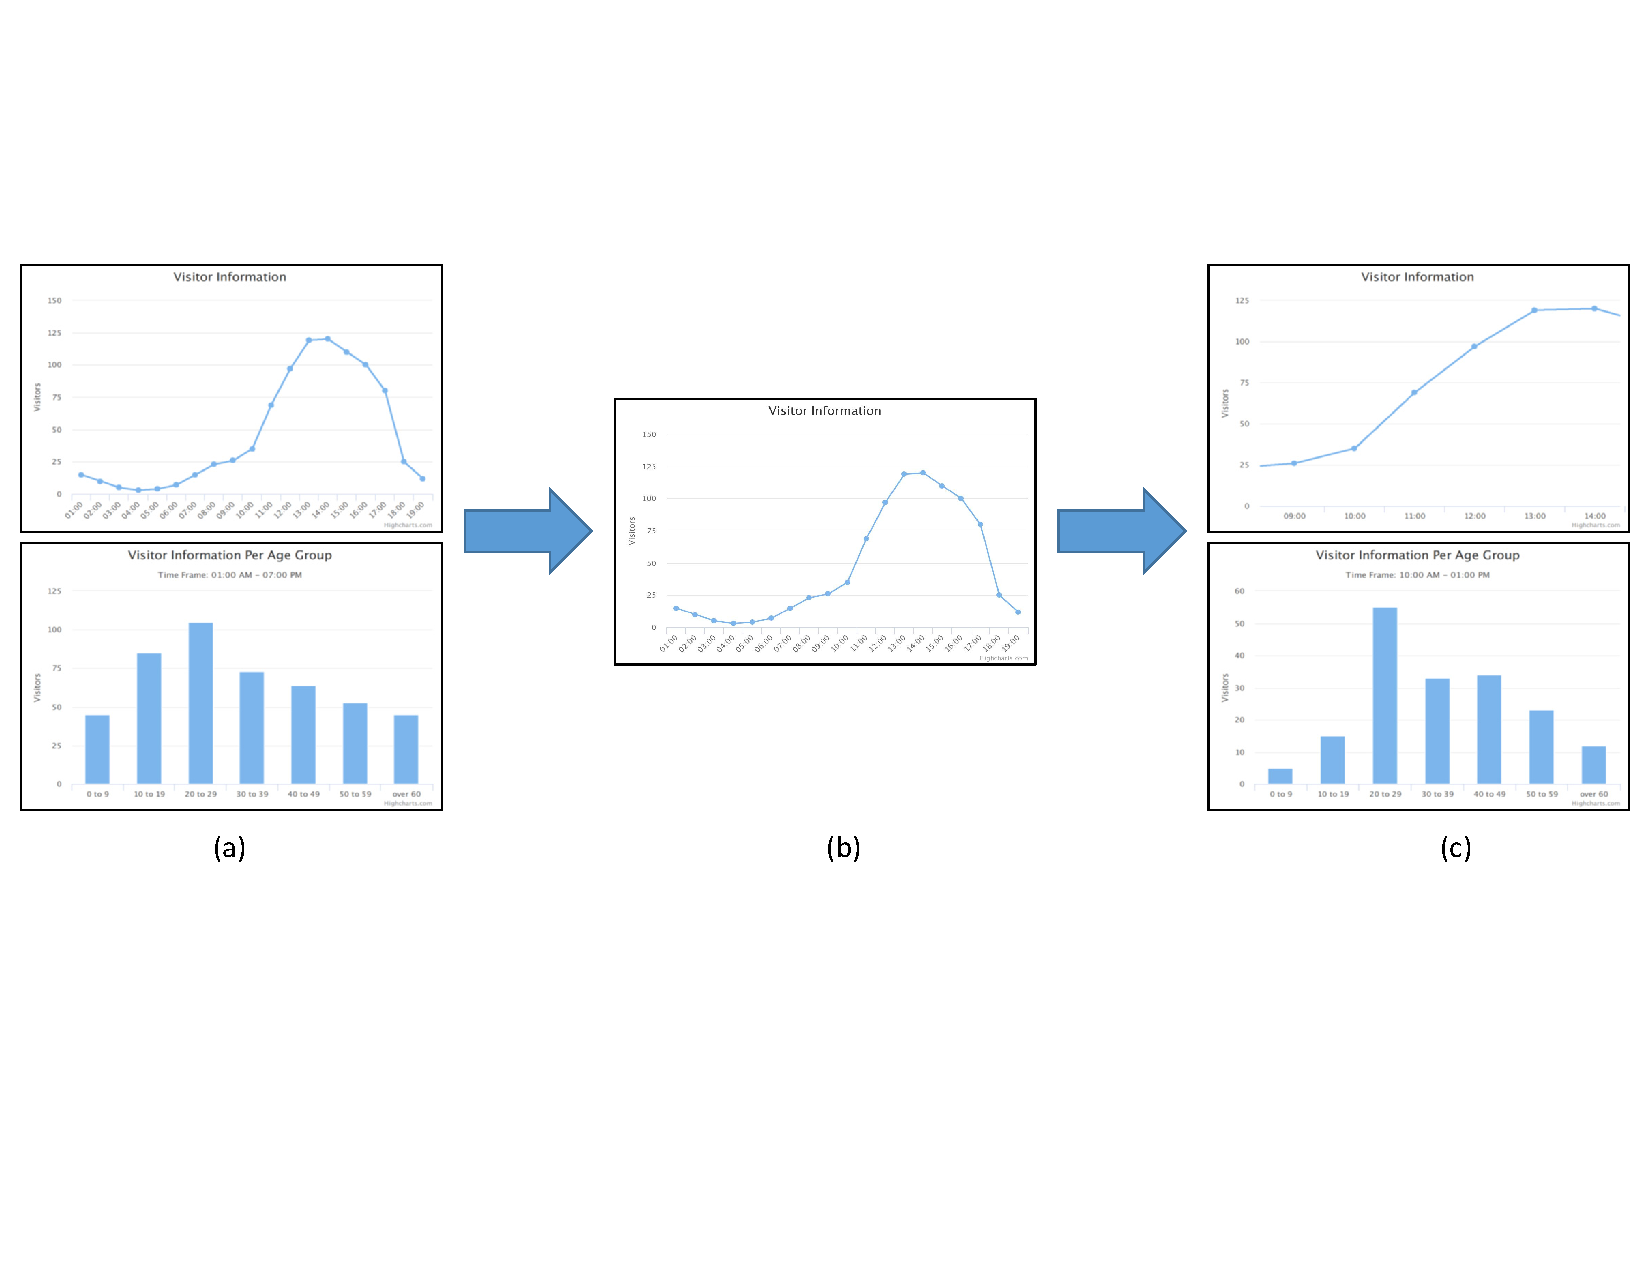
\includegraphics[width=\textwidth]{figures/highchart_final_a.pdf}
	\caption{Demonstration of interactive charts. The analyst's selection automatically updates the second plot (right).}
	\label{fig:vision}
\end{figure*}

\eat{
\begin{figure*}
	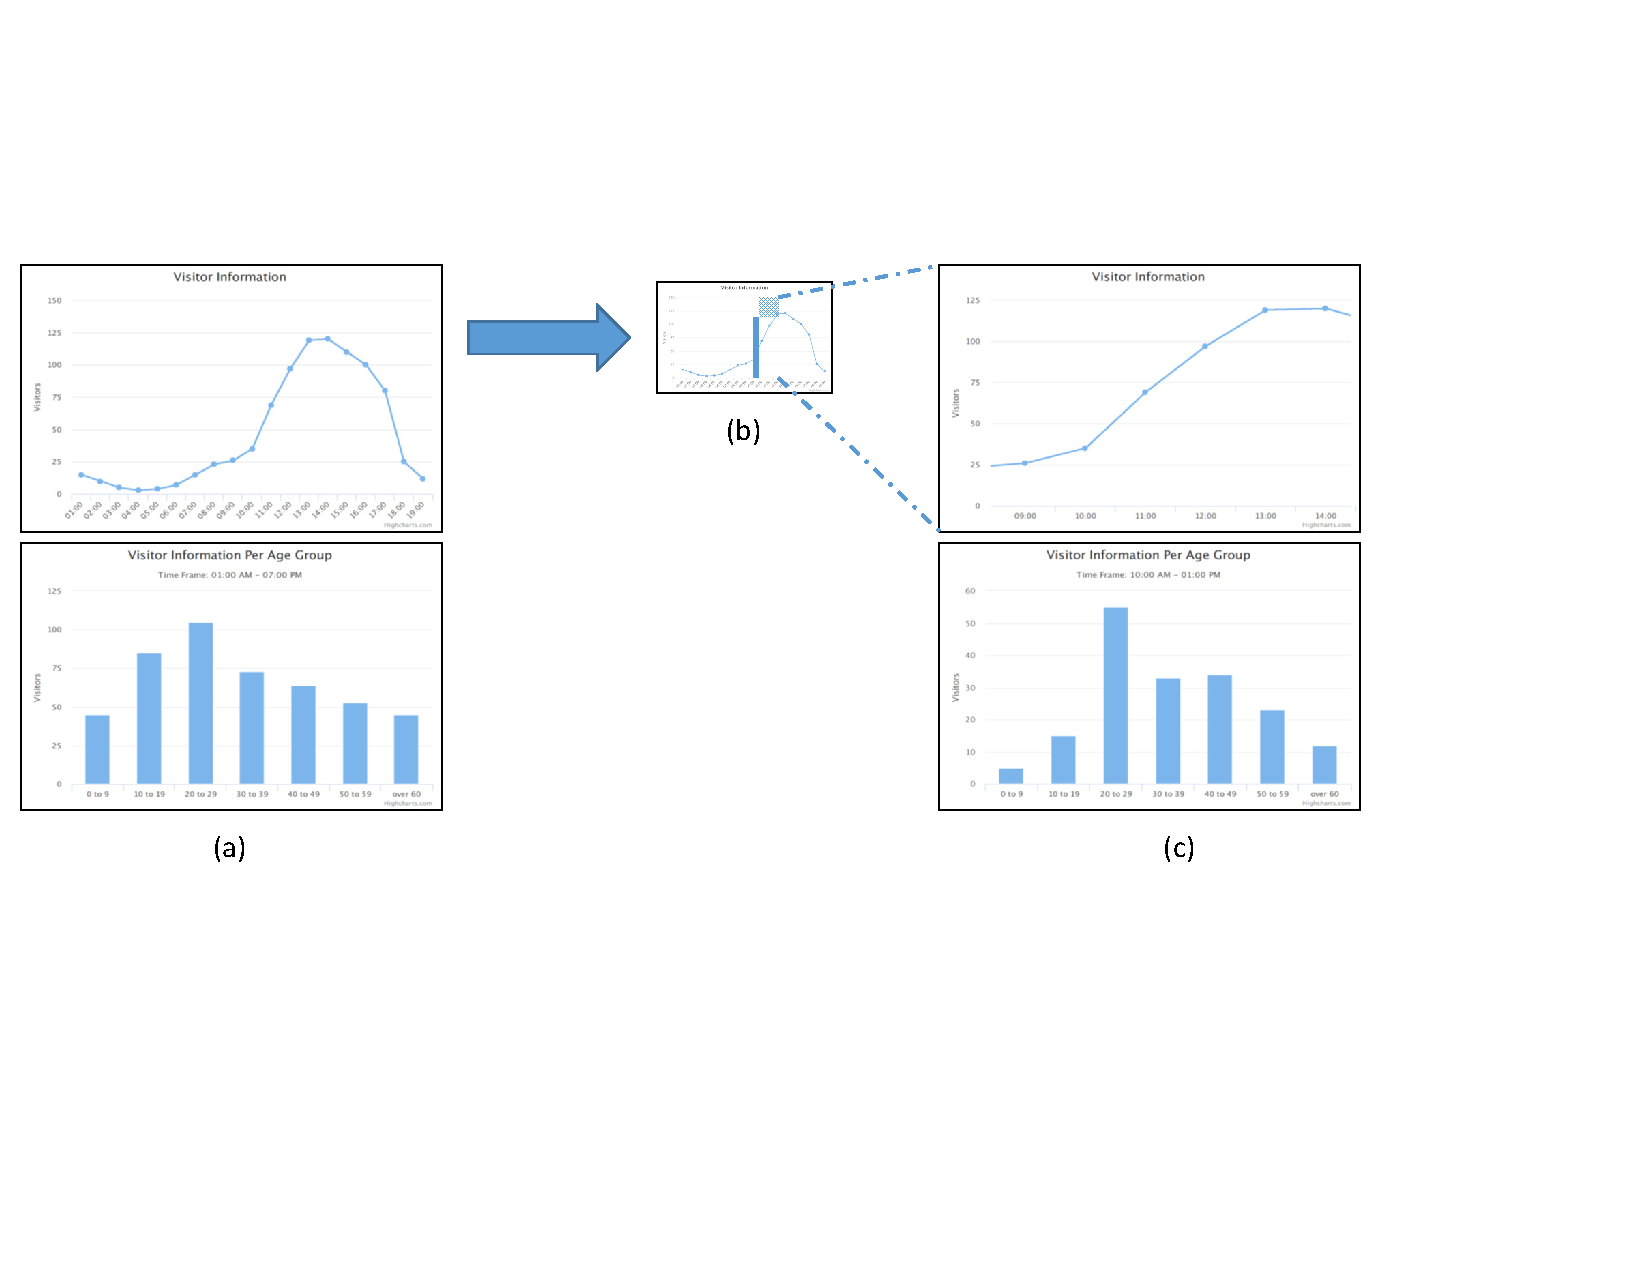
\includegraphics[width=\textwidth]{figures/highchart_final_b.pdf}
	\caption{Demonstration of interactive charts. The analyst's selection automatically updates the second plot (right).}
	\label{fig:vision}
\end{figure*}
}
\eat{
\remark{Ok I thought about it and I propose the following modifications in the paper structure (Nothing major - just moving text around to make it more readable): We begin with a good discussion about the vidette features that can help notebooks in section 2. We then show the entire walkthrough in one section (Section 3). By now, the reader knows what vidette can do so it will be easier to follow and understand the code we show.}
}
 \eat{
We address these issues, by extending interactive notebooks with the  {\projname} framework. {\projname} notebooks support a new template language capable of facilitating common data analysis tasks. The main contributions of this extension are:

\begin{itemize}
	\item \textit{Expressive template language:} Prior work, treats a page as a database view. Building on that, our template language goes beyond SQL query and view definition in both style and fundamental expressiveness. It is a mixture of query as well as web templating language that works on ordered (arrays) and semi-ordered (JSON) data. 
	\item \textit{Easy data retrieval:} Our framework supports communication with all major database types, such as Postgress, MongoDB, SQL etc, eliminating the need for individual DB drivers. Furthermore, using {\projname}, user access credentials for the database server(s) are stored in a configuration file, eliminating the embarassingly insecure practice of typing usernames and passwords in notebook cells vidible to everyone.
	\item \textit{Inline JSON operations:} The primary data structure used in {\projname} is JSON arrays. {\projname} combines the intuitive nature of JSON with the ability to write inline JSON operations, resulting in a clean, structured and readable code.
	\item \textit{Variable binding:} Analysts can easily ``bind'' variables using our template language. ``Binding'', results in automatic re-execution of notebook cells that contain those variables upon a change. {\projname} will trigger execution of the appropriate cells without any extra coding effort. As we show later, combined with inline JSON operations, binding becomes an incredibly versatile tool.

%	\item \textit{Declarative semantics:} {\projname} implements formal declarative \textit{Model-View-View-Model} (MVVM) semantics. \remark{Fill in why this is a good thing. I have no idea.}
%	\item \textit{Expressive template language:} Prior database work, treats a page as a database view. Building on that, our template language goes beyond SQL query and view definition in both style and fundamental expressiveness. It is a mixture of query as well as web templating language that works on ordered (arrays) and semi-ordered (JSON) data. 
%	\item We allow in-line declarative code directly in JSON...
\end{itemize}
}


%In this paper, we demonstrate the use of {\projname} via a walkthrough example. Specifically, we want to use website access data to plot an access count over time histogram. We also want to plot the recorded user demographics (with focus on age groups). We then want to have the ability to interact with the histogram plot and select a time region. This action should automatically update the second plot with the user demographics in the selected time window. 
%
%Without loss of generality, we assume a Jupyter server, where the analysts develop their notebooks and a different database server where data is stored. To retrieve the entirety of the required data, we have to query two different databases and join the returned JSON files. Figure ?? shows how our databases are organized. Our fictional analyst will perform the following high-level tasks:
%
%\begin{itemize}
%	\item Data retrieval from remote databases. 
%	\item Data curation: Join data and prepare for visualization.
%	\item Data visualization.
%\end{itemize}
%
%The remainder of this paper is organized as follows: Sections \ref{section:dataretrieval} -- \ref{section:visualization} present a direct comparison of using {\projname} and an imperative language such as Python in order to complete the tasks of our example. Throughout these sections, we demonstrate some of the main contributions of {\projname}. Section \ref{section:discussion} provides further discussion regarding our proposed extension and presents other useful aspects of it not used in our walkthrough. Finally, Section \ref{section:conclusion} concludes the paper.


\section{Introduction}
\label{section:introduction}

\noindent \textbf{Contributions} We describe the following contributions of \projname:
\begin{compact_item}

%

\item \textit{Declarative Semantics:} We present a formal declarative MVVM semantics for \projname. To the best of our knowledge, this is the first formal presentation of MVVM declarative semantics by an MVVM framework. \yannis{What extra do we offer in light of CIDR11 to the semantics?} 
\costas{Fundamentally, they are both diff driven application frameworks... Some differences are that the CIDR11 and SIGMOD10 version: 1.the template language was written in XML which was more verbose and therefore needed more effort to be written (more characters per line and more total lines of code for the same template instance). 2.Additionally, since template functions were not supported, the app developer often had to inline complex SQL++ queries in the template to ``massage" the data appropriately. 3. Delta functions were not supported. Overall templates appeared more convoluted compared to the current version and therefore they were harder to follow. For more differences check respective file in Notes folder (at the root of the repo)} \yannis{A large difference between CIDR11 and current work is the aim to easily interface with JavaScript. This is behind the functions in the template language, the interfacing of JavaScript components, the JavaScript actions and (the missing) easy programming model for accessing JavaScript data (the latter can stay for journal or OOPSLA)} Hence, the declarative semantics of \projname\ can also serve as an introduction to the semantics of MVVM at large, and to the semantics of \angular\ and other MVVM frameworks, after one accounts for their limitations.
%
\item \textit{Expressive Template Language:} While we draw from prior database research work, which treats the page as a database view, the template language goes beyond SQL query and view definitions in both style and fundamental expressiveness \yannis{Good point for a journal publication but on VLDB suffers from CIDR comparisons. The reason behind the higher expressiveness is new.}: It is a mixture of query language and web templating language that works on ordered data (arrays) and semi-structured data (JSON) \costas{JSON encompasses the concept of arrays/ ordered data}and is expressive enough to cover many common transformations without requiring the use of additional imperative JavaScript code. Notably, it is more expressive than the language of \angular, due to reasons pertaining to differences in their incremental rendering algorithms. \yannis{Cannot be quickly backed up by the example. Two nested loops may be hard but a for/if combo is doable.} \costas{How would it be backed up by example? We would have to introduce Angular and \projname\ templates in the intro, wouldn't we?} Furthermore, besides visualization, the templates can also input data and catch events/activate actions \costas{actions have not been defined}, as a complete web application development framework should do.

%
\item \textit{Incremental Rendering:} The incremental rendering problem has similarities to Incremental View Maintenance (IVM) but also poses distinct new challenges due to (1) template language features that have not received attention by the database community, and (2) unlike IVM whose goal is to update a target materialized view, the incremental rendering algorithm is a \textit{diff propagation} algorithm that results into a sequence of calls to the rendering methods of (the usually 3rd party) components. \yannis{A diff and its resulting rendering method call should have been demonstrated in the context of the example.} Pertaining to Item~(1) \projname\ solves the following diff propagation problems:
\begin{compact_enum}
\item \textit{Handling Arrays:} Arrays are prime citizens of the data model. Therefore we reconsidered what is the appropriate language for describing diffs, so that diffs on arrays are included. \costas{What do we mean when we say ``language" for describing diffs}\yannis{Current example has no motivation for insertion in the middle of array, which is where problems happen.}Second we developed algorithms for propagating such diffs.   
%


\item \textit{Black-box functions in Template:}\yannis{no example of a function either. It need not be the first example but I think there is just no example.} In the rare cases where the out-of-the-box expresiveness of the template language is not enough, the developer can include Javascript function invocations in her template. \projname\ offers a pay-as-you-go approach to the efficient diff propagation through JavaScript functions that may be part of the template: The developer may provide nothing (but the function itself), in which case the diff propagation algorithm will still work but may be slow\costas{Let's avoid the word slow, let's just say it wouldn't work ``incrementally", which is the more efficient.}, as it will be re-evaluating the function. Alternately, the developer may provide one or more diff management functions, which are suggested to her by \projname\ and lead to more efficient diff propagation. \costas{We should also mention that we provide some of these functions out-of-the-box (e.g sortby, groupby etc...)}\yannis{IMPORTANT: we need to discuss how this differs from angular's pay-as-you-go} \costas{Angular does not provide something similar to \projname's delta functions, so there's nothing to pay as you go}
%\costas{The IVM algorithm will be fast, the function re-evaluation may be slow (We should make it clear to the reader that the bottleneck isn't the template IVM algorithm but the user defined function...). That's why we enable the function developer to provide auxiliary delta functions that update the logical page more efficiently. }
%

\item \textit{Loops in Templates} \projname\ provides diff propagation over loop structures.  \costas{Why is that a big deal? This bullet doesn't illustrate why that's challenging or interesting...}\yannis{would be far more convincing with fors and ifs}

% 
\end{compact_enum}
%
The \projname\ incremental rendering also solves the following problems pertaining to its need to translate diffs into rendering method calls. \yannis{as said above, problems should have memorable names and do not repeat the whole description continously} \costas{refer to dictionary spreadsheet} \url{https://docs.google.com/spreadsheets/d/1pn6EPZUnz\_3Tc3e7FnveRxQXcs2uRqD0znERjI0-g0o/edit#gid=0}
\begin{compact_enum}

\item \textit{Easy wrapping of 3rd party components} A novel triggering algorithm enables the easy and pay-as-you-go wrapping of Javascript visualization rendering methods. In particular, the developer in charge of wrapping a visualization component is only tasked with specifying the single diff that a rendering method handles. \costas{This sentence doesn't make sense: ``(The developer specifies the) single diff that a rendering method handles". The developer does not specify diffs, he specifies renderer wrappers and diff signatures (refer to dictionary). The number of renderer wrappers he needs to specify is anything between two (construct-destruct) and the total number of renderers supported by the visualization library} \yannis{Needs example. Recall, earlier we introduced a diff and a corresponding renderer. Here we should change the assumption on renderer or the diff so that we can show simulation.}Therefore the size of the specification \costas{what specification?}is proportional to the number of rendering methods she wishes to wrap, as opposed to the number of the possible kinds of diffs, which is typically far larger. \costas{the latter number is: supported-diff opcodes X potential targets in unit instance} \yannis{tell the number that shows how many diffs exist in our example. You don't have to substantiate yet why so many. The substantiation will come much later once we have shown the unit's "schema" and have explained how many kinds of diff exist.
The most impressive introductions say "without my technique it would be N and with my technique it is M that is an order of magnitude below"} \costas{I don't follow. Why do we need to specify the number of possible diffs. When reading this section it feels like we're comparing our system with a system similar to ours that does not support simulation. Angular does not work with diffs, so this is somewhat pointless.} When a diff is produced that does not correspond directly to a rendering method, \projname\ discovers how to indirectly support it by \textit{simulating} the missing rendering method with existing wrapped rendering methods. \costas{we should add something like: ``This automation significantly simplifies the process of unit wrapping. Since competing frameworks do not provide a similar feature, unit developers are often required to manually perform it manually. This negatively impacts both the amount of time that needs to be spent in unit wrapping and the amount of lines of code that need to be written"}Lines-of-code experiments show the advantage of \projname\ in 3rd party wrapping productivity.

\eat{
\costas{The reasons why Angular directives need more lines are:
Actually the problem, arises when two renderers exist, one at a deeper level then the other. In such cases, Angular directive developers have to install a deep watcher at the higher level and manually compare the parts that correspond to more ``specific" renderers, to identify what changed. This happens to avoid the invocation of multiple renderers, which would be a direct result of}
}
%
\item \textit{Managing Direct Updates and Provenance Heterogeneity} \projname\ treats update diffs as first-class citizens, as opposed to simulating updates by insert-delete combinations. \costas{Not sure why we mention this, Angular directives don't need to simulate updates diffs with insert-delete diffs. Is this something that other IVM algorithms do not support?} This feature leads to higher performance and also superior UI behavior, when the visualization components provide update renderer methods. It also creates a need for keeping track of the provenance of each part of the visualization, so that it can be identified and updated. Notice that provenance has to be converted into terms that the 3rd party component understands, creating a need for special conversion data structures and algorithms. \yannis{Needs support of the example, both on the update and on the provenance. (The current example is an insertion and does not have any provenance problem.)}
\end{compact_enum}
%
\item \textit{Superior performance over other MVVM frameworks:} A net effect of the algorithms is that the client-side incremental rendering algorithm achieves better Big-O algorithmic complexity than the incremental rendering algorithm of \angular\ and also ouperforms it in the presented experiments.
%
\end{compact_item}

{\bf Paper Outline.} \yannisk{Revise after the sections have been finalized} The paper is structured as follows: In Section \ref{section:programming-model} we explain the structure of a \projname\ application as seen by an application developer. Section \ref{section:architecture} describes \projname's internal architecture, while Sections \ref{section:template-ivm}-\ref{section:visual-ivm} describe the incremental view maintenance algorithms that power the framework. Section \ref{section:experiments} compares the performance and productivity gains of the proposed system against the state of the art. Finally, Sections \ref{section:related-work} and \ref{section:conclusion} discuss related work and conclude the paper, respectively.

\section{Conclusion}
\label{section:conclusion}

We presented \projname\ an interactive notebook engine, that enhances interactive notebooks with capabilities that pertain to both data scientist that create notebooks and non-technical notebook readers....

\end{sloppypar}

\bibliographystyle{abbrv}
\bibliography{refs}

\end{document}
